\documentclass{article}
%\usepackage{subfigure}
%\usepackage{subfig}
\usepackage{graphicx} % Required for inserting images
\usepackage{tcolorbox}
\usepackage{subcaption}
\usepackage{tabularx}
\usepackage{amsmath}
\usepackage{mathtools}
\usepackage{subcaption}
\usepackage{xcolor}
\usepackage{amssymb}
\usepackage{booktabs}
\newlength\tindent
\setlength{\tindent}{\parindent}
\setlength{\parindent}{0pt}
\renewcommand{\indent}{\hspace*{\tindent}}
\usepackage[a4paper, top=2cm, bottom=2cm, left=2cm, right=2cm]{geometry}
\usepackage{graphicx}
\tcbuselibrary{minted,breakable,xparse,skins}
\usepackage{subfig}
\setlength{\parindent}{0cm}
  
\title{Global system characterization and analysis}
\author{Matthieu Absil, Ulysse Allard, Hugo Bastin, Kévin Colas, Louis Raviart}
\date{}

\begin{document}

\maketitle

\section{Feuille de route}

\subsection{MCU}
Il faut parler de 
\begin{itemize}
    \item Describe the different components it is composed of : power unit, microphone, memory, ...
    \item Thermal noise, quantization noise, microphone non-idealities (directivity, frequency response,...)
    \item Power consumption 
    \item Check the datasheets to see if there is interesting info   
\end{itemize}

\subsection{Telecom}
\begin{itemize}
    \item Describe the chain : modulation, demodulation (cfo, sto, synchro) 
    \item Measure the range of communication
    \item Check other metrics : SNR, Rx gain needed, BER
    \item Eventually try to measure the efficiency of synchro, sto and cfo correction
\end{itemize}

\subsection{FPGA}
\begin{itemize}
    \item What is accelerated : short/long term sum, complex mag,...
    \item Resource utilization 
    \item Possible additions : other functionalities, trade-offs (in term of resources)
\end{itemize}
\subsection{Characterization}
\begin{itemize}
    \item Identify the limitations/bottlenecks of the system
    \item Performances of the different blocks
    \item Future improvements
\end{itemize}


\section{Introduction}

The world is threatened by the climate change, mostly caused by the industrial revolution, but the resulting technology can be a great tool to mitigate its consequences and protect the Earth. Specifically, we set here our focus on forests, which are essential carbon sinks and biodiversity reservoirs, that are not only threatened by the rise in temperatures that cause an increasing number of fires, but also by illegal deforestation. In this context, the aim of this report is to characterize and analyze an embedded wireless sensing system that performs audio monitoring in natural ecosystems such as forest. This system has for purpose to detect abnormal events, like fires and sawing, compute and extract useful features from those sounds, transmit them through wireless communication to a base station that will identify if an abnormal event is happening. This will allow a faster reaction to better fight the potential threats that the forest is facing and protect it. \\

This report will first present a global system overview that will describe the operating chain and the different blocks that it is made of. In a second time, it will characterize the performances of the actual system based on different criteria such as the classification accuracy or the communication range. It will then identify its weaknesses, limitations and bottlenecks to finally give potential improvements and optimizations that could be conducted in the second part of the project.

\section{System overview}

In order to correctly detect and classify sounds, the system has to follow a specific operating chain that is made of all the necessary steps to ensure a proper audio recording and analysis, a reliable wireless communication and an accurate classification. In this section, we will detail each block composing the chain by briefly presenting their function and their components.  \\

We break down the operation chain in three main fields, the operations executed on the sensor, which is in this application a microcontroller unit (MCU), which have to fit in the limited power available, the telecommunication between the sensor and the classification of the sounds recorded. The chain is made of the following steps : it first acquires the sounds through a microphone and performs a time-frequency analysis to extract features that will be used for the classification. The next step is to transmit the information collected through wireless communication. Finally, on the receiver side, we we demodulate and authenticate the packets received to perform the classification and identify a potential abnormal event.

\begin{figure}[H] %Je referai en bloc en utilisant draw.io si vous voulez
    \centering
    \includegraphics[width=0.95\linewidth]{Plots Rapport final/Schéma blocs/Operating_chain.png}
    \caption{Complete operating chain}
    \label{Complete operating chain}
\end{figure}

We will first describe the operations in the order in which they are carried out. Some of them, as we can see on Figure \ref{Complete operating chain}, are linked to 2 of the fields mentioned, we will of course describe them in only one of the subsections. 

\subsection{MCU operations}

\subsubsection{Microphone interface and sound data acquisition}

The input of this block is the acoustic wave of the sound present in the forest, which will then be transformed into an electrical signal (in Volts) by the microphone to be manipulated on the MCU.
In reality, the amplitude of the signal is really small, in the range of $\mu\text{V}$ or mV. If we use this signal as it is, an issue will appear in the next block when the analog-to-digital converter (ADC) will quantize our signal, as it will not be able to use its whole range of discrete values. This causes to have a higher quantization error and is described in Annex \ref{}. 
To solve this, a Low Noise Amplifier (LNA) is used to amplify the electrical signal in order not add too much quantization noise on the signal. \\

\begin{figure}[h]  % Peut également être modifier
    \centering
    \includegraphics[width=0.5\linewidth]{Plots Rapport final/Schéma blocs/Sound_data_bloc.png}
    \caption{Blocks 1 \& 2 diagram}
    \label{fig:enter-label}
\end{figure}

Another component of this block is an anti-aliasing filter (AAF),  which is a low pass filter used to discard the high frequencies that could create aliasing if they are higher than the sampling frequency of our ADC and do not respect the Shannon-Nyquist theorem. The cut-off frequency of the AAF is $5000$ [Hz], we then sample at a frequency $f_s \geq 2 \cdot 5000$ in order to respect Shannon-Nyquist theorem. In practice, this frequency is $f_s = 11025$ [Hz]. At this point, the signal is made of discrete value in time but not yet in amplitude, this is the role of the ADC that performs the quantization. \\

As for every system, it involves non-idealities. We see from the microphone's datasheet that the frequency response is not constant, which means that we don't have the same amplitude for all the frequency. It has a constant amplitude in the range $[200, 3000]$ [Hz], but it also have an overshoot near to $10$ [kHz] and this overshoot put the amplitude to $7$ [dB] this could be a problem because that could bring us saturation is our signal. \\

\subsubsection{Sound acquisition}

After that the sound signal has been conditioned, this block samples and converts it into discrete 12-bit values that can be handled by the MCU using an ADC. With 12-bit values, it can cover its range, from 0 to 3.3V, with 4096 intermediate values. Of course, the analog signal will rarely be exactly equal to one of these limited values, so the ADC has to round it up to nearest one, which causes a quantization error. This rounding can deteriorate the quality of the signal recorded. \\

Once this is done, the system needs to store the 12 bits computed by the ADC in memory. The memory available in the MCU is given in Table \ref{MCU memory}

\begin{table}[H]
    \centering
    \begin{tabular}{|c|c|c|}
        \hline
        & Flash & RAM \\
        \hline
        Memory in [kBytes] & 1000 & 320 \\
        \hline
    \end{tabular}
    \caption{Memory of the system}
    \label{MCU memory}
\end{table}

Data are stored in the RAM, meaning that everytime we disconnect the board to the alimentation, everytime we discard the data. Our data are stored in a buffer, in reality a big buffer divided in 2 in purpose to run continuously the system. The 12 bits acquired by the ADC represent one sample, this sample is send to the the first buffer, but the buffer is in 16 bits, meaning that we add four 0 at the beginning of the sample to extend it to 16 bits. After that we store it into the first part of the buffer, when this half buffer is full, we're going to process it but we run continuously the system, the sample are so send now to the second half buffer. When it's full, we process it and the sample are sent to the first half buffer etc. If we compute the size of the full buffer, we have :
\begin{equation}
    \frac{320000\cdot 8}{16} = 160000
\end{equation}
This correspond to 80000 samples of audio acquisition because we just have a half buffer at once to store samples.\\
In practice, we can not use the total size of the RAM because the program running on the MCU must have an access to the RAM and also because if we fill too much the RAM, the system could crashed. An estimation of the size of our buffer is 120000 samples ($75 \%$ of the full value). So 60000 samples for an half buffer.

%. It's a small analog signal in volts, to use it, we have so to amplify it and this is made by a LNA (low noise amplifier) in order to add the minimum amount of noise. The AAF (anti aliasing filter) is here to respect the Shannon-Nyquist theorem before the sampling. We have to digitalize this signal to use it in our MCU, this is made by the ADC (analog to digital converter) which sampling and quantize our analog signal.

\subsubsection{Time-frequency analysis and feature extraction}

Once the sounds have been sampled and written in memory, the system needs to transform them into convenient features to be easily handled for the classification. To do so, 
this block computes a time-frequency analysis to obtain melspectrograms, which represent the evolution in time of the frequency content of the sound. The idea is to have access to both information that represent respectively the pitch of the sound (high-pitched or deep) and its rythm (regularity of a chainsaw or singing of a bird). \\

To create the melspectrograms, the signal is first divided into a several subpieces to compute the Fourier transform for each one of them and then concatenate their Fourier transforms to form a spectrogram. One limitation is that these spectrograms represent quite a lot of data to send to the base station, which reduce the performance of the system. To solve this, we use the Mel scale, a non-linear transformation of the frequency scale using overlapping triangular filters. The Mel scale comes from the human perception of sounds that is more sensitive to changes in the lower frequencies than in the higher ones. Because this specific perception comes from a very long evolution, it seems like a good idea to use it as it should in principle allow a better distinction of sounds if evolution did its job correctly. 

\begin{figure}[h]
    \centering
    \includegraphics[width=0.5\linewidth]{Plots Rapport final/Classification/Mel_coeffs.png}
    \caption{Mel filterbanks}
    \label{fig:enter-label}
\end{figure}

To apply this transformation, we use a matrix multiplication of the computed spectrogram by a matrix containing the coefficients that derive from the Mel filterbanks. The result of it is a melspectrogram that will then be transmitted as a feature vector by concatenating the Mel coefficients of each temporal subpiece.

\begin{figure}[h]
    \centering
    \includegraphics[width=0.75\linewidth]{Plots Rapport final/Classification/Spectrogram_to_Melspectrogram.png}
    \caption{Spectrogram and Melspectrogram of the same sound}
    \label{SpecAndMel}
\end{figure}

Currently, the signal is divided into subpieces of 512 samples, and a Fourier transform of 512 is computed for each of these. We use 20 Mel coefficients which allows to reduce the data by $\approx 25$. This compression of the spectral content might cause some imprecision and loss of information, the number of Mel coefficients is a important key parameter of the system and its value can strongly influence its performance.

\subsection{Telecommunication}

\subsubsection{Authentication tag generation}

The MCU needs to transmit the features computed for the classification to the base station. To do so, it cannot simply send the feature vector, but it needs to organise the information as a packet that will not only contains the feature vector but also other fields carrying additional information about the emitter or the integrity of the packet. The information contained in the packets has the following format 
\begin{center}
\texttt{r$\mathbin\Vert$emitter\_id$\mathbin\Vert$payload\_length$\mathbin\Vert$packet\_serial$\mathbin\Vert$app\_data$\mathbin\Vert$tag}
\end{center}
(\texttt{$\mathbin\Vert$} denotes concatenation)
where
\begin{center}
\begin{tabular}{lccl}
    Field & Length (bytes) & Encoding & Description \\ \hline
    \texttt{r} & 1 & & Reserved, set to 0.\\
    \texttt{emitter\_id} & 1 & BE & Unique id of the sensor node.\\
    \texttt{payload\_length} & 2 & BE & Length of \texttt{app\_data} (in bytes).\\
    \texttt{packet\_serial} & 4 & BE & Unique and incrementing id of the packet. \\
    \texttt{app\_data} & any  &  & The feature vectors. \\
    \texttt{tag} & 16 & & Message authentication code (MAC). \\
\end{tabular}
\end{center}

Among these fields, we have the \texttt{emitter\_id}, \texttt{payload\_length} and \texttt{packet\_serial} that are used to describe the packet. A tag is used to ensure the integrity of the communication, and whereas a CRC (Cyclic Redundancy Check) protects only random errors, it also protects against malicious attacks such as MITM and spoofing attacks, where an attacker could try to modify a packet transmitted or impersonate a sensor node and send false information. However, it does not prevent someone to read the packet, but this is not considered a problem for our application as it does not transmit any sensitive information. 
The 16 bytes tag is generated thanks to the CBC-MAC-AES algorithm that is applied on the packet with a secret key $k$ that is decided beforehand and known by both the sender and receiver. 
\[
    \texttt{tag} = \text{CBC-MAC-AES}_{k}\left(
        \texttt{r$\mathbin\Vert$emitter\_id$\mathbin\Vert$payload\_length$\mathbin\Vert$packet\_serial$\mathbin\Vert$app\_data}
    \right)\;,
\]
At the reception, we check that the tag received corresponds to what it should be for the specific packet and the secret key $k$. If not, it could mean that someone is attacking the communication, or simply the packet was corrupted by noise or other technical problems. The effectiveness of the cryptographic function used relies on the high difficulty to invert it, so that the attacker can not find the secret key from the tag. Because of this, if an attacker tries to modify the packet or create one, he does not know which key to use to generate the tag and we will be able to detect it.

\subsubsection{Packet creation}

After that the useful information is added to ensure a safe communication, a packet is created to ensure a functioning wireless communication despite noise and other channel impairments. For this, all packets transmitted have the same following structure 

\begin{figure}[H]  % Peut également être modifier
    \centering
    \includegraphics[width=0.5\linewidth]{Plots Rapport final/Schéma blocs/Packet_Structure.png}
    \caption{Packet structure}
    \label{fig:enter-label}
\end{figure}

with a fixed size of 109 bytes with 100 bytes of useful information (payload). At the beginning of the packet, we find a preamble of 4 bytes as well as a sync word of 4 bytes. At the end, there is 1 byte of CRC to check that the message was not corrupted by random errors. It is used in addition of the authentication tag because it allows a faster detection of random errors, and the tag verification will only be used after to detect malicious errors. \\

The bit rate uses in the system is 50 kHz, we can then find the the packet rate:
\begin{equation}
    \texttt{packet\_rate} = \frac{\texttt{bit\_rate}}{\texttt{packet\_size}} = \frac{50000}{8 \cdot 109} = 57 \hspace{0.1cm} [packet/sec]
\end{equation}

The preamble is composed of a series of "10" sequence and has two main purposes. The first one is to serve as a buffer for the packet detection, as the receiver might not be able to detect exactly the very beginning of the packet and can drop a few bits. The preamble received will then be a bit shorter, which is okay and will still allows it to fulfil its second role. The second purpose is correct the carrier frequency offset (CFO) that can appear between the transmitter and the receiver. 

The sync word is an arbitrarily chosen word that will be used to correct the synchronisation timing offset (STO) to set the same time reference for the transmitter and the receiver. These operations are detailed in the next section.


\subsubsection{Wireless communication}

Once the packets have been formed, the MCU has to transmit them by wireless communication with its S2LP radio. We use here a Continuous Phase Frequency Shift Keying modulation scheme. more specifically a 2-CPFSK. This modulation has for advantage to be non-coherent so it does not need to recover the exact phase, but its bit rate is relatively limited because of its small constellation size. The signal is transmitted and received by two dipole antennas, and is expressed in baseband as 
\begin{equation*}
    e_I(t)\:=\:\exp{\left(j 2\pi I \Delta_f t \right)}\:=\:\begin{cases}
    e_{s_1}(t)\:=\:\exp{\left(j 2\pi \Delta_f t \right)}\:\:\:\text{if}\:\: I=1,\\
    e_{s_0}(t)\:=\:\exp{\left(-j 2\pi \Delta_f t \right)}\:\:\:\text{if}\:\: I=-1,
    \end{cases}
\end{equation*}
where the phase of the signal decreases or increases in function of the symbol sent. \\
The reception is completed by a LimeSDR, a Software-Defined Radio (SDR) board that includes a Field-Programmable Gate Array (FPGA). 

\subsubsection{Packet recovery}
The signal goes first through a LNA and a Low Pass Filter (LPF) to reduce a maximum the impact of the noise. The LPF is a Finite Impulse Response (FIR) composed It then goes to the preamble detection block that will determine if a packet is present and if it is necessary to perform the next steps of the communication chain. It relies on one long-term sum whose purpose is to estimate the energy of the noise in the channel, and a short-term sum whose role is to detect a sudden increase in the energy of the signal. If the short-term sum is higher by a factor K than the long-term sum, it means a packet is present and we can forward it to the rest of the chain. The factor K is an important parameter to set, because if it is too small, we will start to demodulate noise, but if it is too high we will not demodulate any packets. The LPF, energy extraction and soft-thresholding are accelerated in hardware by the FPGA of the LimeSDR. \\

\begin{figure}[H]  % Peut également être modifier
    \centering
    \includegraphics[width=0.8\linewidth]{Plots Rapport final/Schéma blocs/Rx_chain.png}
    \caption{Receiver Chain}
    \label{fig:enter-label}
\end{figure}

%The preamble is here to prevent us from needlessly computing noise and weak signal. It is implemented using 2 sums. A short term sum of 32 word and a long sum of 256 word. The former represent newly received energy and the latter represent the energy over a long time simulating the ambient energy or the noise energy.When the short sum is full is it compared to the long sum. To account the size difference the long sum is first multiplied by K the margin and then divided by 8. If the short sum is at least K time higher than the long sum the signal is forwarded to the rest of the chain, if not we don't compute the signal and the short sum is emptied.\\

If packet is detected, we start processing it to correct the effects of the channel. The chain corrects first the CFO and then the STO. \\
The Carrier Frequency Offset (CFO) is an impairment caused by a small difference between the carrier frequencies $\Delta f_c$ at the Tx and Rx due to variations of the oscillators. This is done by the Moose algorithm that takes a known series of $N$ symbols contained in the preamble. It will estimate the carrier frequency offset based on repetition properties of a training sequence. At first it will use the repetition in the preamble with $N_t = N . R_{RX}$.  So the received sequence can be write like this : 
\begin{equation}
    y[n+N_t] = e^{j2\pi \Delta f_c \frac{N_T\cdot T}{R_{RX}}} \cdot e^{j2\pi \Delta f_c \frac{n\cdot T}{R_{RX}}} \cdot x(\frac{n\cdot T}{R_{RX}}) + w[n + N_t]
\end{equation}
But 
\begin{equation}
    y[n] \approx e^{j2\pi \Delta f_c \frac{n\cdot T}{R_{RX}}} \cdot x(\frac{n\cdot T}{R_{RX}})
\end{equation}
And thus 
\begin{equation}
    y[n+N_t] = e^{j2\pi \Delta f_c \frac{N_t\cdot T}{R_{RX}}} \cdot y[n]
\end{equation}
After using a modified least square problem we can compute the frequency offset
\begin{equation}
    |\widehat{\Delta f_c}| = \frac{arg(\hat{\alpha})}{2\pi \frac{N_t . T}{R_{RX}}}
\end{equation}
However, for a bandwidth B, the maximum CFO that can be corrected is given by  \begin{equation*}
    |\widehat{\Delta f_c}| \leq {\frac{R_{RX}}{2.N_t T}} = \frac{B}{2N}.
\end{equation*}
The metric use to estimate the CFO is the RMSE (Root Mean Square Error). 
We see that there is a trade-off between the precision and the range of the CFO estimation. A large N will improve the precision because because there will be more symbols in the preamble block. More symbols we have, better the estimation is. But since we have a large N, this makes the system less responsive to a large frequency offset. A large frequency offset will cause a phase shift that will accumulate accros the symbols. n other words, the algorithm may become less capable of handling a high CFO when the N increases. And conversely, the system will be less accurate with a small N but the range will be better.
%We use the Moose algorithm. We use a small value of N (number of block on which the algorithm work) to make a precise estimation. Even though this mean it can't correct big offset we have good hardware so it isn't a problem for now.\\

The Symbol Timing Offset (STO) is an impairment coming from the delay accumulated by the received signal which causes not to know the beginning of the packet, and thus the payload, and leads to an incorrect demodulation. To estimate it, we compute the first and second derivative of the phase of the received signal, and we check for abrupt variations that are due to changes of symbol. \\
The demodulation is performed by computing the correlations between the received signal and both symbols of the constellation. We find the corresponding symbol by selecting the one giving the highest, since the symbol should give a correlation equal to 0 as they are orthogonal. \\
The packet parser is here to find the start of the payload. It is done by finding where the sync word, a known sequence, is located inside the packet, and the payload is located after it. \\

The last two things that  we need to take into account in the wireless communication part of the project is the Noise power and the SNR. 

\subsubsection{Authentication tag verification}

The final step of the communication chain, authentication, verify if the demodulated packet is send by our transmitter. If not, the packet is a fake one and the information that it contains is incorrect. This is made by verifying the tag, we have to apply the same algorithm that we have implemented in the generation tag but now in the demodulated message. If the tag generate is the same than the tag in the packet, the packet is verify. 
We have to check that the tag received corresponds to what it should have been with the same message and the shared secret key.

\subsection{Classification}

Once the data is received and verified at the base station, the next step is to identify the sound that was sent by the transmitter. To do this, we use the Mel coefficients contained in the package which capture a compressed version of the sound's spectral and temporal features. These coefficients are passed to a pre-trained classifier model, such as a KNN in our case, which maps them to a set of predefined sound categories, classes. The classifier assigns a probability to each sound class, and multiple methods can be used to determine the predicted label. For instance, the system might select the class that was most frequently chosen in the last 10 packets, or simply choose the class with the highest probability as the predicted sound label.
Our metrics were the accuracy of the classification and the confusion matrix. Accuracy is the proportion of correct classifications over the total number of instances, considering all 5 classes. Confusion matrix offers additional insights into the accuracy metric by showing the number of correct and incorrect classifications for each class.
\begin{figure}[h]
    \centering
      \includegraphics[width=0.2\linewidth]{Plots//Final_reportQ1/RandomConfMatrix.png}
      \caption{Usual Confusion matrix | Accuracy = \frac{\text{Number of correct predictions}}{\text{Total number of predictions}}}
\end{figure}

The difficulty of this part resides in the fact that sounds acquired by the microphone and passed through the AAF are significantly different from real-world sounds. This is because we limit the frequency content to sounds up to 5 [kHz]. As a result, high-frequency components of the original sounds are filtered out, resulting in a loss of informations. Additionally, environmental noise, distortions due to the impulse response of the microphone (attenuated frequencies until 500 Hz), and the lossy compression of Mel coefficients further complicate how the classifier should be trained. Consequently, if we use real data to train the model, it must account for these modifications, as they lead to a representation of the sounds that is quite different from their original, unprocessed forms.\\

So, in order to train the model, even though the dataset contained real-world sounds, we used a technique called data augmentation to try to 
simulate the real world effects on the sounds with echoes, time shift, noise,... As this helps the model to generalize better and to be more robust to the real world sounds.


 
% SECTION
\section{Characterization and analysis}

\subsection{MCU - Embedded software}

The MCU must deliver 1 melspectrogram per series of acquisition. We define 3 important parameters :\\
\begin{table}[H]
    \centering
    \begin{tabular}{|c|c|}
        \hline
        \textbf{SAMPLES PER MELVEC} & 512 \\
        \hline
        \textbf{MELVEC LENGTH} & 20 \\
        \hline
        \textbf{N MELVECS} & 20 \\
        \hline
    \end{tabular}
    \caption{Parameters of a melspectrogram}
    \label{tab:my_label}
\end{table}
%The number of samples per mel vectors :SAMPLES PER MELVEC = 512.\\
%The size of a mel vector : MELVEC LENGTH = 20.\\
%and the number of vector per melspectrogram : N MELVECS = 20.\\
To compute 1 mel vector based on 512 samples we need 123k cycles. At a clock frequency of 48MHz this takes 2.56ms per vector. So at least 51.25 [ms] for computing all vectors.
% 32MHz this takes 3.6ms


\begin{table}[H]
    \centering
    \begin{tabular}{|c|c|c|}
         \hline
         Step Name & Complexity & Percentage of total cycle \\
         \hline
         \hline
         STEP 0.1 Increase fixed-point scale & $\mathcal{O}(n)$ & 3.2 $\%$ \\
         \hline
         STEP 0.2 Remove DC Component & $\mathcal{O}(n)$ & 13.9 $\%$ \\
         \hline
         STEP 1 Windowing of input samples & $\mathcal{O}(n)$ & 3.4 $\%$ \\
         \hline
         STEP 2 Discrete Fourier Transform & $\mathcal{O}(n\log_{}n)$ & 20.2 $\%$ \\
         \hline
         STEP 3.1 Find the extremum value & $\mathcal{O}(n)$ & 13.9 $\%$ \\
         \hline 
         STEP 3.2 Normalize the vector & $\mathcal{O}(n)$ & 13.8 $\%$ \\
         \hline
         STEP 3.3 Compute the complex magnitude & $\mathcal{O}(n)$ & 6.5 - 15.9 $\%$ \\
         \hline
         STEP 3.4 Denormalize the vector & $\mathcal{O}(n)$ & 5.6 $\%$ \\
         \hline 
         STEP 4 Apply MEL transform & $\mathcal{O}(n^3)$ & 18.2 $\%$ \\
         \hline
         %PLLs & 1 / 1 (100\%) \\
         %\hline
    \end{tabular}
    \caption{Complexity of the different features}
    \label{complexity}
\end{table}

For the step 3.3 (compute the complex magnitude) there can be a high variation of cycles due to numerous uses of divisions operation that aren't done in constant cycles. Divide need between 2 and 12 cycles depending of the data.\\\\
If we regard into the other functions doing by the MCU, we have the following execution time :
\begin{table}[!h]
    \centering
    \begin{tabular}{|c|c|c|}
        \hline
        Function & number of cycle & time execution [ms] \\
        \hline
        Packetizing & 4380k & 91.2 \\
        \hline
        Radio transmission & 6 630k & 138.1 \\
        \hline
    \end{tabular}
    \caption{Execution time of the other main functions}
    \label{tab:time autre fonctions}
\end{table}\\
The most part of the execution time of the Packetizing is the calculation of the tag, which take $99 [\%]$ of the packetizing.\\
In order to know which function is the "bottleneck" or the \textit{hard real-time} of our MCU, we have to increase their execution time, this can be made by decreasing the clock of our MCU :
\begin{table}[!h]
    \centering
    \begin{tabular}{|c|c|c|c|c|c|c|}
        \hline
        & Full Features calculation & [ms] & Packetizing & [ms] & Radio transmission & [ms] \\
        \hline
        Clock at 32 [MHz] & 123 & 76.9 & 4375 &  & 4430 &  \\
        \hline
        Clock at 16 [MHz] & 123 & 153.8 & 4378 &  & 2240 &  \\
        \hline
        Clock at 8 [MHz] & 123 & 307.5 & 4393 &  & 1147 &  \\
        \hline
        Clock at 4 [MHz] & 124 & 615 & 4422 &  & 604 &  \\
        \hline
        Clock at 2 [MHz] & 125 & 1230 & 4481 &  & 331 &  \\
        \hline
    \end{tabular}
    \caption{Number of kcycles}
    \label{tab:my_label}
\end{table}\\

%4349811/4350510

If we build the projet into \textit{STM32CUBE}, we can observe the memory used for the code :
\begin{table}[H]
    \centering
    \begin{tabular}{|c|c|c|}
        \hline
        & Default builder & Optimizer for size build \\ 
        \hline
        Flash memory & 140.59 [kB] (13.73$\%$) & 126.35 [kB] (12.34 $\%$) \\
        \hline
        RAM & 21 [kB] (6.56 $\%$) & 20.59 [kB] (6.56 $\%$) \\
        \hline
    \end{tabular}
    \caption{Memory usage}
    \label{tab:my_label}
\end{table}
We see so that the memory won't be a limitation in the future of our project because we won't write 10 times more code for the future of the project.\\\\


% SECTION
\subsection{Characterization of the classification model}
We chose a \textbf{k-Nearest Neighbors (KNN)} model with $k=8$ and $n=14$ for classification based on the grid-search below. 
To evaluate the model, we used two metrics: \textbf{Accuracy}, which measures the proportion of correct classifications over the total number of instances, considering all 5 classes, and the \textbf{Confusion Matrix}, which offers additional insights into the accuracy metric by helping to identify underperforming classes or confusion between similar categories. Indeed, accuracy was chosen as the main metric because it provides a simple way to measure how many samples were correctly classified, giving a clear idea of the model's overall performance. The confusion matrix was also used to better understand where the model makes mistakes, such as which classes are being confused with each other. This is particularly useful in multi-class classification tasks, where accuracy alone might not reveal issues like class imbalance or class similarity. These metrics were selected because they are easy to use and interpret while providing a good balance of understanding the model's overall performance and identifying areas for improvement. 
\begin{figure}[h]
    \centering
    \includegraphics[width=0.3\linewidth]{Plots//H5_plots/K_N_tuning.png}
    \caption{KNN and PCA hyperparameters accuracy heatmap}

\end{figure}
\\
The dataset was divided into training (70\%) and testing (30\%) sets using \textit{stratified sampling} to ensure that the class distribution remained consistent across both splits. Indeed, random split should provide a nearly balanced set but with stratify makes sure that the class distribution is balanced. To further evaluate the model and reduce the risk of overfitting, we applied \textit{5-fold Stratified Cross-Validation} on the training set. This approach ensures that every sample is included in both training and validation phases at least once, providing a reliable measure of the model's ability to generalize to unseen data. 
\begin{figure}[h]
    \centering
    \includegraphics[width=0.5\linewidth]{Plots/Final_reportQ1/dataug.png}
    \caption{Possible sound transformations}
    \label{fig:enter-label}
\end{figure}
Additionally, We used data augmentation techniques such as adding background noise, echo, time shift, and random noise to improve the robustness of our classification model, but not scaling as this will be explained later. Data augmentation, because of the fact that the model was primarily trained on clean audio samples from the original dataset, is crucial as it simulates real-world conditions, helping the model handle variations in input data caused by environmental factors or due to the microphone noise and/or non-linear distortions. By introducing more variability, augmented data makes the classification task more challenging, allowing the model to generalize better and perform more reliably on noisy, inconsistent real-world data. Consequently, the model becomes more robust and capable of handling noisy, imperfect data.
\subsubsection{New dataset and augmentation}

The original dataset is made of high quality sounds, each during 5 seconds, but this is actually quite far from the actual sounds we will try to classify. In practice, we are able to record sounds of 950 ms (to 950 [ms] to compute every mel vectors) and those sounds will be corrupted by various effects caused by the electronics or the environment. For those reasons, we would like to create a new dataset that is closer to the reality in the field. Initially, in order to build the feature vector, we take the original sounds as it is and we only take the first 950 ms so that we have the desired number of columns for our melspectrograms. Each melspectrogram is a $20 \times 20$ matrix where the number of rows corresponds to the number of mel coefficients and the number of columns retained, corresponding to the duration of the recording, is determined by the following formula: 
\begin{equation}
    n_{\text{columns}} = \frac{\text{Duration} \times \text{Sr}}{\text{NFT} \times 1000}
\end{equation}

With \textbf{Duration} is the length of the sound in milliseconds, \textbf{Sr} is the sample rate (in Hz)
and \textbf{NFT} is the number of frames used in the Fourier Transform. The feature vector for a single sound is then obtained by stacking the 20 columns of the melspectrogram into a single column vector, resulting in an array of 400 features. The dataset of sounds provided consists of 5 classes, with 40 sounds per class, giving 200 sounds in total. By applying the above process, we construct a new dataset represented as a $200 \times 400$ matrix, where each row corresponds to the feature vector of one sound for a certain label. Now, in order to have a dataset closer to reality, we can artificially add imperfections to the sounds. The possible transformations are time shifting, scaling, echo, background sound and noise and are represented in the figure below.
\begin{figure}[h]
    \centering
    \begin{subfigure}[b]{0.54\linewidth}
        \centering
        \includegraphics[width=\linewidth]{Plots/Final_reportQ1/mismatch.png}
        \label{fig:mm}
    \end{subfigure}
    \hfill
    \begin{subfigure}[b]{0.44\linewidth}
        \centering
        \includegraphics[width=1\linewidth]{Plots/H5_plots/Sound_transformations.png}
        \label{fig:dataaug}
    \end{subfigure}
\end{figure}


For our new dataset, we did not apply scaling because we train our model with normalized sounds thus their amplitude should not affect the classification. We applied noise, background sound and echos as the sounds that the MCU will record will have the same effects. 
We also applied time shifting, because the sound recording can take place at any time and the time reference should not impact the prediction. When we applied data augmentation through noise addition, it was crucial to maintain a consistent logic regarding the amount of noise added (defined by its standard deviation) to achieve a realistic final SNR. Thus, we set a minimum SNR of 20 dB, which corresponds to a moderately noisy environment (typically between 15 and 25 dB). To determine the noise's standard deviation, we analyzed the signal power across all classes and opted for the median instead of the mean, as the mean is biased by high-energy sounds. We chose the median power of the "fire" class ($\sigma^2 = 0.000805$), which had the lowest power, and adjusted the noise's standard deviation ($\sigma = 0.0284$) to meet the target SNR.

\begin{table}[h!]
    \centering
    \begin{tabular}{ccc}
        \toprule
        \textbf{Normalization Method} & \textbf{Mean Accuracy (\%)} & \textbf{Std Deviation (\%)} \\
        \midrule
        L1 Norm         & 65.6 & 1.8 \\
        L2 Norm         & 66.9 & 1.4 \\
        Divide by max   & 67.6 & 1.6 \\
        \bottomrule
    \end{tabular}
    \caption{Mean accuracy and standard deviation for different normalization methods for 100 classifications on the provided audio set}
    \label{tab:normalization_comparison}
\end{table}

Also, we used normalization (divide by max) before training and testing (indeed, if we normalize the training set, we need to normalize testing set to be consistent) because in this audio classification the amplitude of the sound can vary significantly between samples. Normalization ensures that all feature vectors are scaled consistently, preventing features with larger amplitudes from dominating the model's decision process. Moreover, tests were made on the different type of normalization and we finally used the "divide by max" normalization in order to enhance our classifier in terms of accuracy.


% \begin{table}[h!]
% \centering
% \begin{tabular}{|c|c|c|c|c|}
% \hline
% \textbf{Threshold} & \textbf{Mean Acc (No Th)} & \textbf{Mean Acc (Th)} & \textbf{Std Dev (No Th)} & \textbf{Std Dev (Th)} \\ \hline
% 0 $\sigma$ & 0.6288 & 0.6455 & 0.0350 & 0.0348 \\ \hline
% 1 $\sigma$ & 0.6293 & 0.6555 & 0.0341 & 0.0339 \\ \hline
% 2 $\sigma$ & 0.6286 & 0.6507 & 0.0345 & 0.0320 \\ \hline
% 3 $\sigma$ & 0.6315 & 0.6370 & 0.0342 & 0.0331 \\ \hline
% \end{tabular}
% \caption{Impact of thresholding on accuracy and standard deviation}
% \label{tab:threshold_impact}
% \end{table}
% pas sur de cette partie


Finally, using these transformations on the dataset, in order to span all the corrupted sounds that could be recorded by the MCU, we have a new dataset of 1000 feature vectors, each made of 400 features, that should better represent reality on which we used our classifier model for training and evaluation. This larger, augmented dataset should not only allow the model to better generalize to real-world conditions but also helps mitigate the risk of overfitting by introducing more variability into the training process. Consequently, the model's performance on unseen, noisy, and imperfect data is improved as we can see in the figure below.

\begin{figure}[h]
    \centering
    \includegraphics[width=0.25\linewidth]{Plots//Final_reportQ1/lastaccuracyconfusion.png}
    \caption{Mean accuracy : 69.9$\%$ |
Std deviation in accuracy : 4.3$\%$}
\end{figure}

We see that it manages to classify the sounds with an accuracy that depends on the sound subclass. In the case of chainsaw or handsaw sounds,the classifier has sometimes trouble to distinguish them. The classifier has also trouble to distinguish helicopters and chainsaw because their respective melspectrograms may be too similar in some cases but this will be covered in more detail in the section on time frequency content.

\subsubsection{Classification using the MCU}
In order to test on 50$\%$ of the sound, a python script was playing 20 sounds of a certain class in a row and every second an acquisition was made. It means that there is 100 acquisition per class so 500 in total when we tested with the jack. For testing with the micro, the same procedure was applied, but instead of playing individual sounds, we used the LELEC210X YouTube playlist as the source. Since the audio quality and conditions differed when using the micro, we limited the number of acquisitions to 25 per class, leading to a total of 125 test acquisitions. While this reduced dataset is smaller, it still captured the same performance trends observed with the jack but with worsened accuracy.
\begin{table}[h!]
    \centering
    \begin{tabular}{lcccc}
        \toprule
        \textbf{Method} & \textbf{Naive} & \textbf{Majority Voting} & \textbf{Average Feature} & \textbf{Maximum Likelihood} \\
        \midrule
        \multicolumn{5}{l}{\textbf{Jack's Results} } \\
        Provided set accuracy (\%)     & 31.20 & 30.11 & 31.20 & 32.00 \\
        New set accuracy (\%)         & 29.47 & 25.60 & 29.47 & 28.00 \\
        Accuracy Drop (\%)            & 1.73  & 4.51  & 1.73  & 4.00 \\
        \midrule
        \multicolumn{5}{l}{\textbf{Micro's Results}} \\
        Provided set accuracy (\%)     & 18.40 & 23.20 & 18.40 & 22.40 \\
        New set accuracy (\%)         & 14.40 & 21.60 & 14.40 & 15.20 \\
        Accuracy Drop (\%)            & 4.00  & 1.60  & 4.00  & 7.20 \\
        \bottomrule
    \end{tabular}
    \caption{Comparison of accuracy with jack and micro using the provided set/new set i.e. LELEC210X YouTube playlist}
    \label{tab:jack_mic_comparison}
\end{table}

Indeed, the classifier struggles to generalize well, as evidenced by the accuracy drop between the provided dataset and the new dataset, particularly for sounds recorded with the micro. This poor generalization comes firstly from the fact that the dataset is insufficient. While the model was trained on clean, high-quality audio samples, these do not adequately reflect the diversity or imperfections of real-world recordings even with the data augmentation.
In order to look at the poor generalization of the classifier, another way is to see why is looking at the confusion matrix. Below, We can see that the accuracy is even more class dependant for every tests done. In the best-case scenario, with 100 classifications of per class,  the model performs well on chainsaw sounds as well as birds sounds, has a mediocre performance for the handsaw class but can't recognize 2 classes, such as crackling fire and helicopters. In the worst-case scenario with only 25 classifications per class, the model describes the same trends but with results that are worse than random.

\begin{figure}[H]
    \centering
    \begin{subfigure}{0.4\linewidth}
        \centering
        \includegraphics[width=0.75\linewidth]{Plots/Final_reportQ1/bestconfu.png}
        \caption{Confusion matrix for the best case (20 sounds per classes)}
    \end{subfigure}
    \centering
    \begin{subfigure}{0.4\linewidth}
        \centering
        \includegraphics[width=0.75\linewidth]{Plots/Final_reportQ1/worstconfu.png}
        \caption{Confusion matrix for the worst case (5 sounds per classes)}
    \end{subfigure}    
\end{figure}

Previously a significant issue is the timing of sound recordings. If the sound was recorded at a moment with limited or no useful information, the model could have misclassify the sample because it lacked the critical features needed for accurate identification. One potential solution to mitigate this issue is to incorporate a temporal memory of recent sound recordings. In order to improve the classification, 4 methods were tested.\\
Naive Method involved classifying each recording independently without using any memory information. Majority Voting combined predictions from multiple recordings by choosing the class that appeared most often in the 5 last acquisitions. The third method, Average Feature, averaged predict probability of the features last 10 features. Maximum Likelihood method takes into account the probabilities of all predictions over time and selects the class that is most likely based on the overall pattern. 

\subsubsection{Time frequecy content of the melspectrograms \& non idealities}

In order to know why our classify has , we have trained our classification model with the original sounds of the dataset. These sounds are of relatively high quality compared to the sounds acquired directly by the MCU. In practice, the acquisition chain of the MCU is made of several non-idealities and imperfections. The signal received is for example affected by thermal noise, quantization noise or echo and background noise, and the melspectrogram will consequently differ from the one coming from the original "perfect" sound. We will compare for different sounds the melspectrograms coming from the original sound and from the jack and the microphone.

\begin{figure}[H]
    \centering
    \begin{subfigure}{0.35\linewidth} % Slightly larger width for the first figure
        \centering
        \includegraphics[width=1.2\linewidth]{Plots/H5_plots/birds2_python.png}
        \caption{Birds - Original dataset}
    \end{subfigure}
    \hfill
    \begin{subfigure}{0.27\linewidth} % Smaller width for the second figure
        \centering
        \includegraphics[width=\linewidth]{Plots/H5_plots/birds2_jack.png}
        \caption{Bird sound acquired with jack from MCU}
    \end{subfigure}
    \hfill
    \begin{subfigure}{0.27\linewidth} % Smaller width for the third figure
        \centering
        \includegraphics[width=\linewidth]{Plots/H5_plots/birds2_micro.png}
        \caption{Birds sound acquired with micro from MCU}
    \end{subfigure}
    \caption{Comparison of bird sounds from the original dataset and  acquired via jack and micro from the MCU.}
\end{figure}

We can see that we are doing an acquisition from around 3.5 to around 4.5s.

\begin{figure}[H]
    \centering
    \begin{subfigure}{0.35\linewidth} % Slightly larger width for the first figure
        \centering
        \includegraphics[width=1.2\linewidth]{Plots/H5_plots/chainsaw12_python.png}
        \caption{Chainsaw - Original dataset}
    \end{subfigure}
    \hfill
    \begin{subfigure}{0.27\linewidth} % Smaller width for jack-acquired figure
        \centering
        \includegraphics[width=\linewidth]{Plots/H5_plots/chainsaw12_jack.png}
        \caption{Chainsaw sound acquired with jack from MCU}
    \end{subfigure}
    \hfill
    \begin{subfigure}{0.27\linewidth} % Smaller width for micro-acquired figure
        \centering
        \includegraphics[width=\linewidth]{Plots/H5_plots/chainsaw12_micro.png}
        \caption{Chainsaw sound acquired with micro from MCU}
    \end{subfigure}
    \caption{Comparison of chainsaw sounds from the original dataset and  acquired via jack and micro from the MCU.}
\end{figure}

We can see that we are doing an acquisition from around 2.5 to around 3.5s.

\begin{figure}[H]
    \centering
    \begin{subfigure}{0.35\linewidth} % Slightly larger width for the first figure
        \centering
        \includegraphics[width=1.2\linewidth]{Plots/H5_plots/helicopter0_python.png}
        \caption{Helicopter - Original dataset}
    \end{subfigure}
    \hfill
    \begin{subfigure}{0.27\linewidth} % Smaller width for jack-acquired figure
        \centering
        \includegraphics[width=\linewidth]{Plots/H5_plots/helicopter0_jack.png}
        \caption{Helicopter sound acquired with jack from MCU}
    \end{subfigure}
    \hfill
    \begin{subfigure}{0.27\linewidth} % Smaller width for micro-acquired figure
        \centering
        \includegraphics[width=\linewidth]{Plots/H5_plots/helicopter0_micro.png}
        \caption{Helicopter sound acquired with micro from MCU}
    \end{subfigure}
    \caption{Comparison of helicopter sounds from the original dataset and acquired via jack and micro from the MCU.}
\end{figure}
We can see that we are doing an acquisition from around 0.5 to around 1.5s but only via the jack.
\begin{figure}[H]
    \centering
    \begin{subfigure}{0.35\linewidth} % Slightly larger width for the first figure
        \centering
        \includegraphics[width=1\linewidth]{Plots/Melspectrogram/fire10.png}
        \caption{Fire - Original dataset}
    \end{subfigure}
    \hfill
    \begin{subfigure}{0.27\linewidth} % Smaller width for the second figure
        \centering
        \includegraphics[width=\linewidth]{Plots/Melspectrogram/firejack10.png}
        \caption{Fire sound acquired with jack from MCU}
    \end{subfigure}
    \hfill
    \begin{subfigure}{0.27\linewidth} % Smaller width for the third figure
        \centering
        \includegraphics[width=\linewidth]{Plots/Melspectrogram/firemic10.png}
        \caption{Fire sound acquired with micro from MCU}
    \end{subfigure}
    \caption{Comparison of fire sounds from the original dataset acquired via jack and micro from the MCU.}
\end{figure}
We can easily see that we are doing an acquisition from around 1.8 to around 2.8s.
\begin{figure}[H]
    \centering
    \begin{subfigure}{0.35\linewidth} % Slightly larger width for the first figure
        \centering
        \includegraphics[width=1\linewidth]{Plots/Melspectrogram/handsaw10.png}
        \caption{Handsaw - Original dataset}
    \end{subfigure}
    \hfill
    \begin{subfigure}{0.27\linewidth} % Smaller width for the second figure
        \centering
        \includegraphics[width=\linewidth]{Plots/Melspectrogram/handsawJack2.png}
        \caption{Handsaw sound acquired with jack from MCU}
    \end{subfigure}
    \hfill
    \begin{subfigure}{0.27\linewidth} % Smaller width for the third figure
        \centering
        \includegraphics[width=\linewidth]{Plots/Melspectrogram/handsaw10mic2.png}
        \caption{Handsaw sound acquired with micro from MCU}
    \end{subfigure}
    \caption{Comparison of Handsaw sounds from the original dataset and  acquired via jack and micro from the MCU.}
\end{figure}
We can see that we are doing an acquisition from around 0.5 to around 1.5s but only via the jack.\\
Gaussienne due to the microphone? Attenuation of low frequencies? Amplitude?


In this study, we trained our classification model using high-quality sounds from the original dataset. However, in real-world scenarios, sounds acquired via the MCU are affected by various non-idealities, such as thermal noise, quantization noise, echo, and background noise. These imperfections lead to melspectrograms that differ significantly from the ones generated from the original, "ideal" sounds. Below, we discuss key observations based on the comparison of melspectrograms from the original dataset and those recorded by the MCU (via jack and microphone).

\begin{itemize}
   % \item \textbf{Signal Duration:} The original dataset contains sounds that are 5 seconds long, whereas the MCU records much shorter segments (approximately 950 [ms] to compute every mel vectors). This duration mismatch can complicate classification, as the recorded segment might not always include relevant features required for accurate identification.
    \item \textbf{General Differences:} Melspectrograms from MCU-acquired sounds are typically less accurate due to hardware limitations and environmental factors. Recordings made via the jack are generally less corrupted than those made using the microphone, as jack recordings are not influenced by external disturbances, such as echoes or background noise.
    
    \item \textbf{Bird Sound:} The jack and microphone recordings capture identifiable portions of the original signal. However, the microphone melspectrogram exhibits additional spectral content, likely caused by sound propagation through the air or the quality of the playback equipment used during recording.
    
    \item \textbf{Chainsaw Sound:} The melspectrogram from the jack recording closely resembles the original, whereas the microphone recording shows significant deviations. These deviations make it more difficult to extract features resembling the original sound.
    
    \item \textbf{Helicopter Sound:} The jack recording produces a melspectrogram that is fairly similar to the original, with only minor discrepancies. In contrast, the microphone recording is heavily corrupted, likely due to louder background noise or other environmental imperfections.
\end{itemize}

In summary, the shorter duration and non-idealities of MCU-acquired sounds considerably affect the quality of the resulting melspectrograms. While jack recordings tend to generate melspectrograms that are closer to the original, microphone recordings are more susceptible to corruption due to environmental disturbances. In some cases, the acquired sounds still retain sufficient information for classification, but in others, the corruption is too severe to provide a meaningful representation of the original sound.

One major limitation is the lower quality of the sounds recorded by the MCU, which introduces distortions and noise that degrade the input data. Unfortunately, improving the quality of the recorded audio is constrained by the hardware limitations of the MCU. 

\newpage
\section{Power Consumption Analysis}

The power consumed by the MCU is a critical aspect of the system as its only source of power is the light energy gathered by its solar panel. In this section, we wish to characterize the energy consumption of each block and their associated tasks to identify the bottlenecks that could reduce the system's performances.

\subsection{General power consumption}

For the application, the sensor should continuously listen to the environment and send the processed information to the base station. The power profile of this continuous operation is a repetition of the same cycle composed of audio acquisition, packet creation and wireless transmission.

\begin{figure}[h]
    \centering
    \begin{subfigure}{0.49\linewidth}
        \centering
        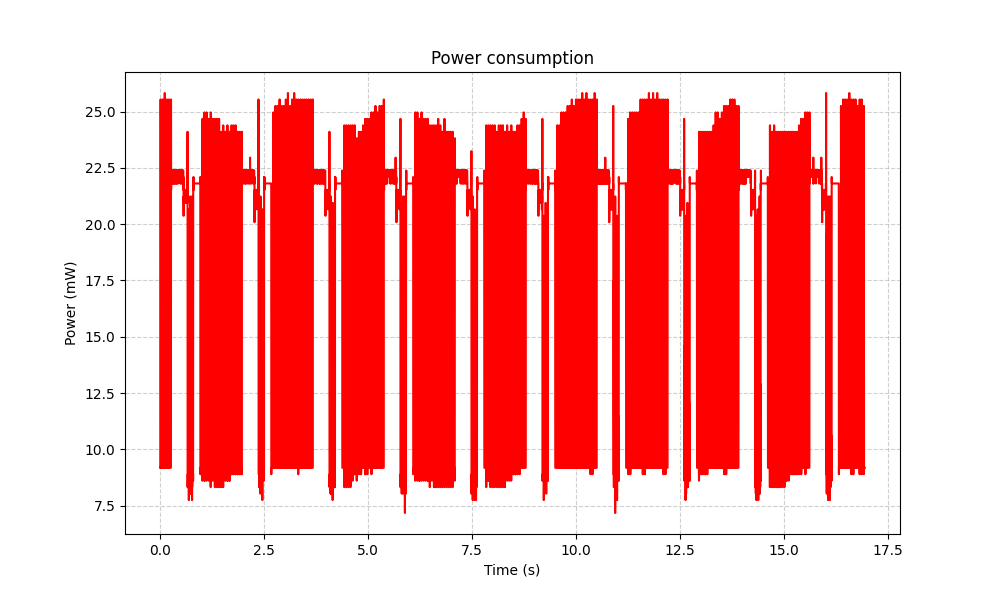
\includegraphics[width=\linewidth]{Plots Rapport final/Power Consupmtion/Power_Usage_MCU.png}
        \caption{Power profile of the sensor}
    \end{subfigure}
    \hfill
    \begin{subfigure}{0.49\linewidth}
        \centering
        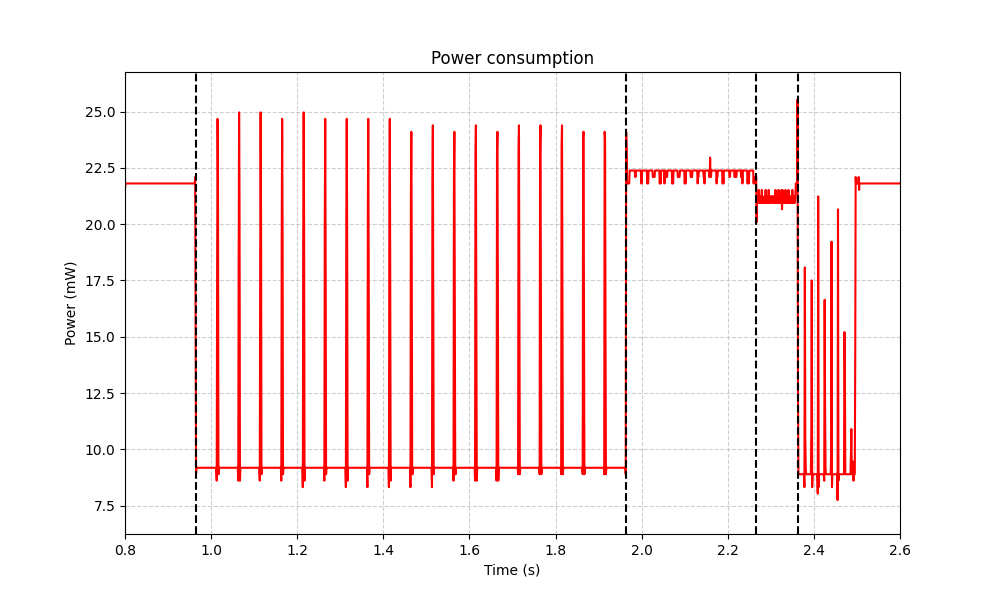
\includegraphics[width=\linewidth]{Plots Rapport final/Power Consupmtion/Power_Usage_MCU_Zoom_V4.png}
        \caption{Power consumption for 1 cycle}
    \end{subfigure}
\end{figure}


At the very start and very end,the system active but waiting a event.\\
We can see there is 3 distinct part :\\
The first part is the audio acquisition and computing of the mel vectors. Only the AFE and ADC are working but they wake up the CPU when enough data is ready. Once it finished computing, it goes back to WFI, this explain the spikes. (CPU duty cycle ?).\\

The second part is the packetization and tag computation. Only the CPU is required here.\\

The third part is the transmission of all the data. This part is short as a lot of effort was put in reducing total data size.\\

% PV cells IndoorLightSeries.pdf
% FIND THE RIGHT ONE
A requirement of the application is its ability to maintain operability while power by a PV cell. TO DO


\subsection{AFE power consumption}

The Analog Front End is here to manage the analog treatment of the signal and bring it to an ADC for later computation.

\begin{figure}[H]
    \centering
    \includegraphics[width=0.8\linewidth]{Plots Rapport final/Power Consupmtion/Power_Usage_AFE_V1.png}
    \caption{Graph of power consumption of the AFE}
\end{figure}

We can see on that it consummation is constant but rise when acquiring data. The spikes are finger's snap and the other one is a random noise. The dynamic consummation is quite high as it goes near or above static one in both case\\
The AFE is made of 3 modules, the microphone, a Low Noise Amplifier (LNA) and a Low Pass Filter LPF. Of respective consumption 16µA, 20µA and 0µA as it is a RC cell. This way different that what we found in practice. 

% ALI/AOP MCP6321
% TYP 20 µA de conso 
% Micro ICS-40310
% TYP 16 µA (but between 10 and 25)
% LPF
% Cellule RC d'après la board schematics

\subsection{Radio power consumption}

PLOT GRAPH
COMPARE TO DATA SHEET

\section{Conclusion}

\section{Bibliographies}

% ADC 5.33 Msps maximum conversion rate with full resolution and Down to 18.75 ns sampling time
% STM32L4A6ZG_datasheet.pdf
% Cortex-M4 instruction refernece manuel
%https://developer.arm.com/documentation/ddi0439/b/CHDDIGAC#ftn.CHDCBDIC

\end{document}


% Possibilité Améloiration
% Réduire la frequence du CPU
% Control de gain automatique
% Control de K
% CFO plusieur test avec Grand N et petit N
